\documentclass[Rapport/Rapport_main.tex]{subfiles}
\begin{document}
\section{Kravspecifikation}


\subsection{Funktionelle krav}
I dette afsnit beskrives de funktionelle krav, hvilke aktører der er indeblandt, og hvordan CarnGo applikationen fungerer.

\subsubsection{Aktør beskrivelse}

For at afklare hvilke aktører, der anvender og interagerer med CarnGo, er der udarbejdet et aktør-kontekst diagram. Dette kan ses i figur \ref{fig:actor_context}
\begin{figure}[H]
    \centering
    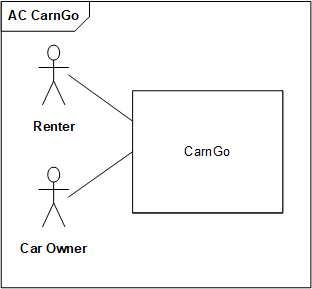
\includegraphics[width=0.5\textwidth]{Kravspecifikation/Funktionelle_krav/ActorContext/graphics/AC_CarnGo.png}
    \caption{Aktør-kontekst diagram for CarnGo}
    \label{fig:actor_context}
\end{figure}

I \ref{fig:actor_context} ses de to primære aktører Car Owner, og Car Renter. Begge primær aktører er brugere af CarnGo applikationen, dog har de to aktører forskellig funktionalitet. Car Owner har mulighed for at sætte biler til leje, mens Renter ikke kan sætte biler til leje, men kun leje biler til eget brug.
Nu hvor Aktørerne til systemet er kendt, kan der i de næste afsnit kigges på User stories for applikationen. 

\newpage
\subsubsection{User Story}
User stories forklarer ud fra brugernes perspektiv, hvordan brugeren kan benytte de diverse funktionaliteter i applikationen. User stories viser, hvordan brugeren interager med appliktationen, og derved bliver user stories abstrakte.

Der blev valgt at lave user stories istedet for use cases, fordi use cases er meget omfattende og forklarer fuldt hvert brugsscenario. Det betyder kravspecifikationen vil kræve mere tid, og derved have mindre tid på implementerering af produktet.       

User stories for Car'n'Go er opsummeret i et story map i figur \ref{fig:Story_map}. Første række angiver epics, dvs. de kategorier som systemets user stories falder ind under. For hver epic er der således en til flere relaterede user stories, som er listet vertikalt. Det er intentionen, at de bliver mere specialiserede, som man bevæger sig nedad. Placeringen af den enkelte user story har dog ingen betydning for dens prioritet.

---------------REF--------------

\begin{figure}[H]
    \centering
    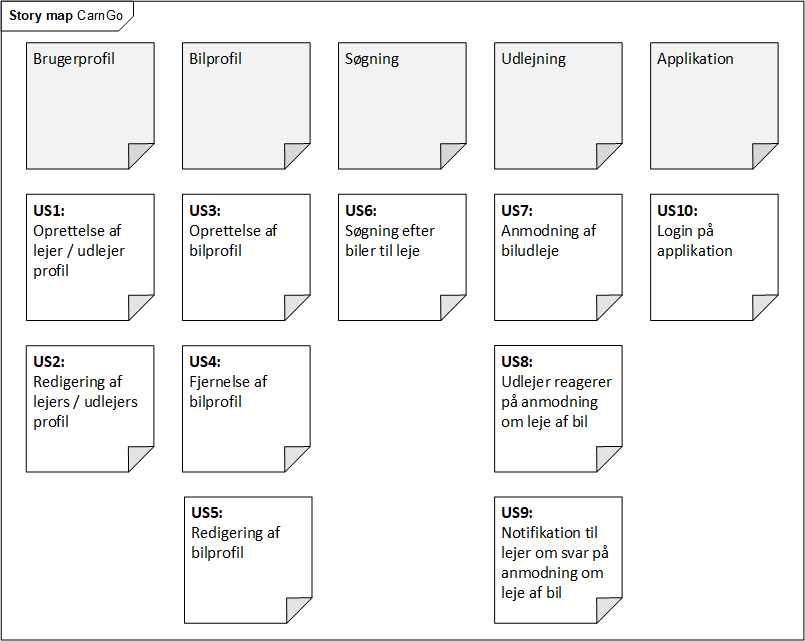
\includegraphics{Kravspecifikation/Funktionelle_krav/UserStories/graphics/Story_map.png}
    \caption{User Story Map}
    \label{fig:Story_map}
\end{figure}

Som der kan ses i figur \ref{fig:Story_map} er der fem epics og 10 user stories. De 10 User stories bliver kort beskrevet nedenunder. Den fulde beskrive af de forskellige user stories kan findes i afsnit Actor Context, i bilag Kravspecifikation.
 ------------ Der skal ref ordenligt her, når vi kan ---------------


\subsubsection{Oprettelse af profiler}

User stories indenfor dette epic beskriver, hvordan en bruger kan interagere med sin profil, og hvordan oprettelsen af den foregår. Denne epics funktionalitet er det første en bruger kommer til at interagere med i applikationen. 

\textbf{US 1: Oprettelse af lejer/udlejer profil}

Denne userstory beskriver hvordan man kan oprette en profil, samt også bestemme hvilken slags profiltype det skal være. Det kan enten være en Lejer- eller udlejerprofil. 

\textbf{US 3: Oprettelse af bilprofil}

User story 3 forklarer, hvordan en bruger kan oprette en bilprofil til brugeren bil.


\subsubsection{Redigering/ fjernelse af profiler}

User stories inden for dette epic beskriver, hvordan bruger med en udlejerprofil kan interagere med sine bilers profiler.

\textbf{US 2: Redigering af lejers/udlejers profil}

Denne userstory beskriver fortæller hvordan kunden kan ændre sin profil, således hvis noget af sin information er blevet forældet, kan det blive ændret til det rigtige.

\textbf{US 4: Fjernelse af bilprofil}

User story 4 forklarer, hvordan en bruger kan fjerne en af sine eksternede bilprofiler. 

\textbf{US 5: Redigering af bilprofil}

User story 5 forklarer, hvordan en bruger kan redigere sine bilprofiler, hvis der er noget information som er forældet og derved skal opdateres.

\textbf{US 10: Fjernelse af bruger profil}

User story 4 forklarer, hvordan en bruger kan slette sin profil fra applikationen. 


\subsubsection{Søgning}

\textbf{US 6: Søgning efter biler til leje}

User story 6 omhandler, hvordan en bruger med lejerprofilen kan søge efter biler. Brugeren har mulighed for at indtaste søgekriterier, som f.eks. ønsket tidsinterval og forskellige bilattributter.  

\subsubsection{Udlejning}
User stories inden for dette epic beskriver, hvordan udlejnings processen fungerer mellem udlejer og lejer.  

\textbf{US 7: Anmodning af biludleje}

User story 7 viser interaktionen mellem udlejer og lejer, når lejen anmoder biludleje på en bilprofil. Når der bliver anmodet biludleje på en af udlejerens biler, får biludlejen en notifikation. Udlejeren kan enten godkende udlejen eller afvise udelejen. 

\textbf{US 8: Notifikation til lejer om svar på anmodning om leje af bil}

User story 8 omhandler når lejeren har anmodet at leje en bil. Lejeren får en notifikation tilbage, som viser udlejens respons, som enten kan være at afvise eller godkende.   

\subsubsection{Applikation}
\textbf{US 9: Login på applikation}

User story 9 viser hvordan en bruger kan logge ind på applikationen, med enten sin udlejer- eller lejerprofil.




\newpage
\subsection{Ikke-Funktionelle krav}

De vigtigste ikke-funktionelle krav bliver beskrevet i dette afsnit. Disse krav har fulgt FURPS modellen og MoSCoW-prioritering. Fuld beskrivelse af ikke funktionelle krav findes her: ------------- REF ----------.


\textbf{Functionality}
\begin{itemize}
    \item CarnGo applikationen skal aldrig fryse, dvs. ophøre med at respondere på brugerens input, i mere end 3 sekunder af gangen (Must)
    \item CarnGos knapper skal reagere, når der bliver sluppet på knappen (Should)
    
\end{itemize}


\textbf{Usability}
\begin{itemize}
    \item CarnGos typografi skal ha et kontrastforhold over 4.5:1 for å følge  \href{https://www.w3.org/TR/UNDERSTANDING-WCAG20/conformance.html#uc-levels-head}{WCAG AA standarden} (Must)
\end{itemize}


\textbf{Reliability}
 \begin{itemize}
     \item CarnGo skal håndtere 10 aktive brugere af applikationen på samme tid (Should)
     \item CarnGo skal håndtere 20 inaktive brugere af applikationen på samme tid (Should)
 \end{itemize}


\textbf{Performance}
\begin{itemize}
    \item CarnGo skal være klar til brug inden for 10 sekund efter, at applikationen åbnes (Must)
\end{itemize}


\textbf{Maintainability}
\begin{itemize}
    \item CarnGo's GUI kode skal følge et GUI design pattern, der gør det nemt at overføre til andre platforme (Must)
    \item CarnGo skal kunne tilgås på en PC med internet forbindelse og Windows 10 OS (Must)
\end{itemize}


\textbf{Security}
\begin{itemize}
    \item CarnGo skal censurere brugerens password, når der logges ind på applikationen (Must)
\end{itemize}



\end{document}